\documentclass[aspectratio=169]{beamer}
\usepackage{graphicx}
\usepackage{amsmath}
\usepackage{amsthm}
\usepackage{amssymb}
\usepackage{natbib}
\usepackage[T1]{fontenc}
\usepackage[utf8]{inputenc}
\usepackage[english]{babel}
\usepackage{bm}
\usepackage{hyperref}
\usepackage{xcolor}
\usepackage{booktabs}
\usepackage{soul}
\usepackage{algorithm2e}

\newcommand{\bruno}[1]{\textcolor{blue}{#1}} % Bruno Sanso edits- blue
\newcommand{\findcite}{{\color{red} [Find Citation]}}
\newcommand{\needcite}{\findcite}
\newcommand{\makenote}[1]{{\color{red} #1}}
\newcommand{\Chi}{\mbox{\Large$\chi$}}
\newcommand{\norm}[1]{\left\lVert #1 \right\rVert}
\newcommand{\inorm}[1]{\norm{#1}_{\infty}}
\newcommand{\pnorm}[2]{\norm{#1}_{#2}}
\newcommand{\prob}[1]{\text{Pr}\left[#1\right]}
\newcommand{\expect}[1]{\text{E}\left[#1\right]}

\newtheorem{prop}{Proposition}

\DeclareMathOperator{\tr}{Tr}
\DeclareMathOperator*{\argmin}{arg\,min}
\DeclareMathOperator*{\argmax}{arg\,max}

\usetheme{Berlin}
\setbeamertemplate{navigation symbols}{}
\setbeamertemplate{mini frames}{}
\setbeamertemplate{footline}{}
\renewcommand*{\slideentry}[6]{}

\bibliographystyle{plainnat}

\makeatletter
\newlength{\frameheadheight}
\setlength{\frameheadheight}{2cm}
\newlength{\frametextheight}
\setlength{\frametextheight}{\paperheight}
\addtolength{\frametextheight}{-\footheight}
\addtolength{\frametextheight}{-\headheight}
\addtolength{\frametextheight}{-\frameheadheight}
\makeatother

\setcounter{tocdepth}{1}

\title{Inference for multivariate peaks-over-threshold models}
\author{Peter Trubey}
\institute{Bruno's Lab Meeting}
\date[12/6/2021]{Dec. 6, 2021}

\begin{document}

\begin{frame}[plain]
  \titlepage
\end{frame}

\section{Introduction}
\begin{frame}
  \frametitle{Multivariate peaks-over-threshold models}
  \begin{itemize}
    \item $\bm{Z} \in {\mathbb R}^d_+ = [0,+\infty)^d\backslash[\bm{0},\bm{1}]$,
    \item Assume existence of limiting measure $\mu$ such that
      \[
        \lim\limits_{n\to\infty}n\prob{\frac{1}{n}\bm{Z}\geq \bm{z}} =
         \mu\left([\bm{0},\bm{z}]^c\right),
      \]
    %   \begin{itemize}
    %     \item $\mu$ is distribution of $\bm{Z}$ in extreme regions
    %     \item The \emph{Exponent} measure
    %   \end{itemize}
    \pause
    \item We can factorize $\mu$ into
      \[
        \mu\left( \left\lbrace\bm{Z} : \bm{V} \in A , R > r\right\rbrace \right) =
         r^{-1}\Phi(A).
      \]
      where $R(\bm{Z}) = \max_{\ell}Z_{\ell}$, \; $V(\bm{Z}) = \frac{\bm{Z}}{R(\bm{Z})} \in {\mathbb S}_{\infty}^{d-1}$
    %   \begin{itemize}
    %     \item $R \in (1,\infty)$ is the radial component, and
    %     $\bm{V} \in {\mathbb S}_{\infty}^{d-1}$ the angular component of $\bm{Z}$
    %   \end{itemize}
    \end{itemize}
\end{frame}

\begin{frame}
    \frametitle{Modelling multivariate PoT}
    \begin{enumerate}
        \item Standardize marginal components such that $Z_{\ell}\mid Z_{\ell > 1} \sim \text{Pareto}(1)$
        \item Transform $Z$ to independent $R$, $\bm{V}$
        \item distribution of $\bm{V}$ $\longrightarrow$  dependency structure of $\bm{Z}$
    \end{enumerate}
\end{frame}

\section{Methodology}
\subsection{Data Processing}
\begin{frame}
  \frametitle{Data processing}
  \begin{enumerate}
    \item Fit GP parameters marginally
      \begin{itemize}
        \item threshold $b_{t,\ell} = \hat{F}_{\ell}^{-1}\left(1 - \frac{1}{t}\right)$
        \item $a_{\ell}$, $\xi_{\ell}$ fit by ML on threshold exceedences.
        % "nothing more permanent than a temporary solution"
      \end{itemize}
    \item Standardize the data
      \[
        z_{i\ell} = \left(1 + \xi_{\ell}\frac{w_{i\ell} -
         b_{t,\ell}}{a_{\ell}}\right)_{+}^{1/\xi_{\ell}}
      \]
    \item Keep where $r_i = \max_{\ell}z_{i\ell} > 1$
    \begin{itemize}
      \item decluster?
    \end{itemize}
  \end{enumerate}
\end{frame}

\subsection{An angular distribution}
\begin{frame}
  \frametitle{The Unit $\mathcal{L}_p$ Sphere ${\mathbb S}_p^{d-1}$}
  \begin{figure}
     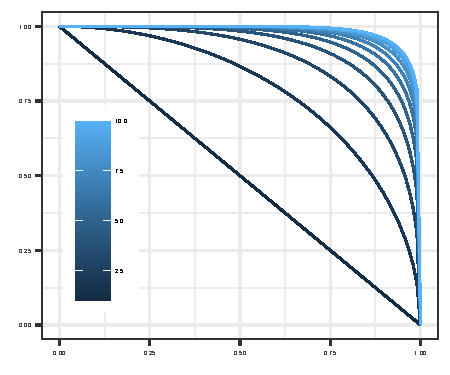
\includegraphics[width=0.475\textwidth]{./images/p_sphere}
     \hfill
     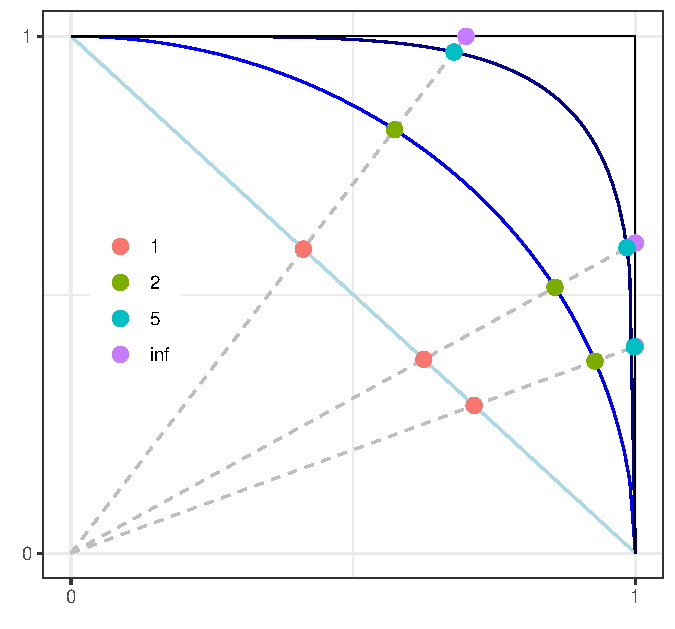
\includegraphics[width=0.475\textwidth]{./images/p_project}
  \end{figure}
\end{frame}

\begin{frame}
  \frametitle{Projecting a distribution onto the unit sphere}
  \small
  \begin{itemize}
    \item the $\mathcal{L}_p$ norm \[
        \lVert \bm{s} \rVert_p = \left({\textstyle\sum}_{\ell = 1}^d
          \lvert s_{\ell}\rvert^p\right)^{\frac{1}{p}}
      \]
    \item Let $y_d = \left(1 - {\textstyle\sum}_{\ell = 1}^{d-
      1}y_{\ell}^p\right)^{\frac{1}{p}}$
    \item Then
      \[
        T(x_1,\ldots,x_d) = \left(\pnorm{\bm{x}}{p},
          \frac{x_1}{\pnorm{\bm{x}}{p}}, \ldots ,
          \frac{x_{d-1}}{\pnorm{\bm{x}}{p}}\right) = (r,y_1,\ldots,y_{d-1})
      \]
    is intertible with
      \[
        T^{-1}\left(r,y_1,\ldots,y_{d-1}\right) =
          \left(ry_1,\ldots,ry_{d-1}, r\left(1 -
            {\textstyle\sum}_{\ell = 1}^{d-
            1}y_{\ell}^p\right)^{\frac{1}{p}}\right)
      \]
    \item The determinant of the Jacobian takes the form
      \[
        r^{d-1}\left[\left(1 - {\textstyle\sum}_{\ell = 1}^{d
          -1}y_{\ell}^p\right)^{\frac{1}{p}} +
          {\textstyle\sum}_{\ell = 1}^{d-1}y_{\ell}^p\left(1 - {\textstyle\sum}_{l=1}^{d-1} y_{\ell}^p\right)^{\frac{1}{p} - 1}\right]
      \]
      % Incidentally, we can't use this to form a distribution on
      % S_{\infty}^{d-1} as the transformation is not differentiable.
      % So -- model on S_p^{d-1} for some large p, then do model evaluation
      % on S_{\infty}^{d-1}
    \end{itemize}
\end{frame}

\begin{frame}
  \frametitle{Projected Gamma Family}
  \begin{itemize}
    \item Product of independent Gammas
      \[
        f(r,\bm{ y}) = \prod_{\ell = 1}^{d}
          \left[\frac{\beta_{\ell}^{\alpha_{\ell}}}{
            \Gamma(\alpha_{\ell})}(ry_{\ell})^{\alpha_{\ell} - 1}
            \exp\lbrace-\beta_{\ell}ry_{\ell}\rbrace\right]
        \times r^{d-1}\left[y_d +
              {\textstyle \sum}_{\ell = 1}^{d-1}y_{\ell}^p\left(y_d^p\right)^{\frac{1}{p} - 1}\right]
      \]
    \item integrate out $r$ yields \emph{Projected Gamma} family
      \[
        \text{PG}(\bm{ y}\mid\bm{ \alpha},\bm{ \beta}) =
            \prod_{\ell = 1}^d\left[
            \frac{\beta_{\ell}^{\alpha_{\ell}}}{\Gamma(\alpha_{\ell})}
                  y_{\ell}^{\alpha_{\ell} - 1}\right]
        \times \left[y_d +
            {\textstyle \sum}_{\ell = 1}^{d-
            1}y_{\ell}^p\left(y_d^p\right)^{\frac{1}{p} - 1}\right]
        \times \frac{\Gamma({\textstyle\sum}_{\ell =
         1}^d\alpha_{\ell})}{\left({\textstyle\sum}_{\ell = 1}^d
                      \beta_{\ell}y_{\ell}\right)^{{\scriptstyle\sum_{\ell =
                       1}^d \alpha_{\ell}}}}
      \]
      defined for $\bm{y}\in {\mathbb S}_p^{d-1}$, and for finite $p>0$.
  \end{itemize}
\end{frame}

\begin{frame}
  \frametitle{Dirichlet Process Mixture of Projected Gammas}
  \begin{itemize}
    \item Using Projected Gamma as a kernel distribution
      \[
       \bm{y}_i \sim \text{PG}(\bm{y}_i|\bm{\theta}_i) , \;\;\; \bm{\theta}_i \sim G, \;\;\; G \sim \mathcal{DP}(\eta, G_0)
      \]
    \item Create Variants using forms of $G_0$ and associated priors
      \begin{itemize}
        \item PG--G
          \[
            G_0 = \mathcal{G}(\alpha_{j1}\mid\xi_1,\tau_1)\prod_{\ell = 2}^d\mathcal{G}(\alpha_{j\ell}\mid\xi_\ell,\tau_\ell)\mathcal{G}(\beta_{j\ell}\mid\zeta_\ell,\sigma_{\ell})
          \]
          with Gamma priors on $\xi_\ell$, $\tau_{\ell}$, $\zeta_{\ell}$, and $\sigma_{\ell}$.
        \item PG--LN
          \[
            G_0 = \mathcal{LN}(\bm{\alpha}_j\mid \bm{\mu},\bm{\Sigma})\prod_{\ell = 2}^d\mathcal{G}(\beta_{j\ell}\mid\zeta_{\ell},\sigma_{\ell})
          \]
          with Normal prior on $\bm{\mu}$, Inverse Wishart prior on $\bm{\Sigma}$, and Gamma priors on $\zeta_{\ell}$, and $\sigma_{\ell}$.
        \item PRG--G and PRG--LN when $\beta_{j\ell} := 1$
      \end{itemize}
  \end{itemize}
\end{frame}

\section{Evaluation}
\subsection{Scoring rules}
\begin{frame}
  \frametitle{Scoring Rules}
  \begin{itemize}
    \item Posterior Predictive Loss
      \[
        S_{\text{PPL}}\left(P,\bm{x}_i\right) =
          \frac{1}{d}\sum_{\ell = 1}^d\left[\text{Var}_P\left(X_{i\ell}\right) +
          \left(\text{E}_P\left[X_{i\ell}\right] - x_{i\ell}\right)^2\right]
      \]
    \pause
    \item Energy Score
      \[
        S_{\text{ES}}\left(P, \bm{x}_i\right) =
          \text{E}_P g\left(\bm{X}_i, \bm{x}_i\right) -
          \frac{1}{2}\text{E}_P g\left(\bm{X}_i,\bm{X}_i^{\prime}\right)
      \]
      where $g$ is a negative definite kernel
  \end{itemize}
\end{frame}

\subsection{A Negative Definite Kernel}

\begin{frame}
    \frametitle{Inadequacy of Euclidean Distance}
    \begin{columns}[T] % align columns
    \begin{column}{.60\textwidth}
    \centering
    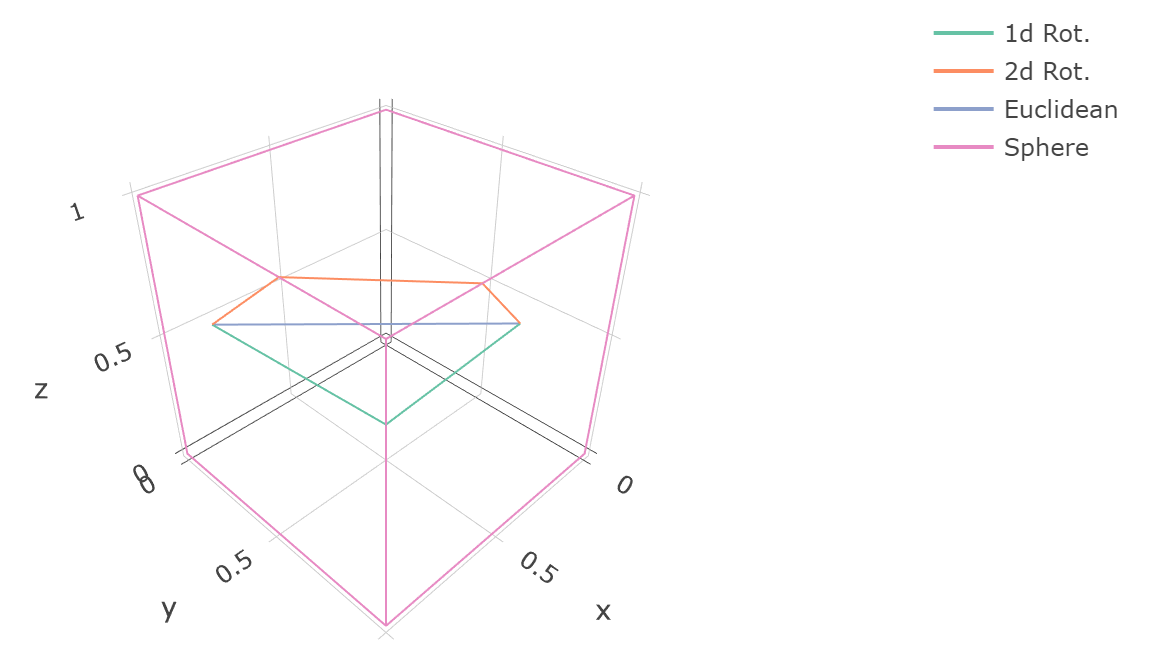
\includegraphics[width=\linewidth]{./images/rotation}
    \end{column}%
    \hfill
    \begin{column}{0.4\textwidth}
    \begin{itemize}
      \item Euclidean norm will under-report distance between $\bm{a}$ and $\bm{b}$
      \pause
      \item Distance is difficult on ${\mathbb S}_{\infty}^{d-1}$
        \begin{itemize}
          \item What path is optimal?
          \item $\sum_{k = 0}^{d-2}\binom{d-2}{k}$ possible paths!
        \end{itemize}
      \item A cheaper way?
    \end{itemize}
    \end{column}
    \end{columns}
\end{frame}

\begin{frame}
  \frametitle{A negative definite kernel for ${\mathbb S}_{\infty}^{d-1}$}
  \begin{prop}
    For points $a,b \in {\mathbb S}_{\infty}^{d-1}$ the kernel defined as
    \[
      g(\bm{a},\bm{b}) = \begin{cases}
        \pnorm{\bm{b}-\bm{a}}{2} &\text{ if }\argmax_{\ell}\bm{a} =
        \argmax_{\ell}\bm{b}\\
        \pnorm{\bm{c}-\bm{a}}{2} + \pnorm{\bm{b}-\bm{c}}{2} &\text{ otherwise}
      \end{cases}
    \]
    where $c$ is in the intersection of the faces corresponding to $\bm{a}$
    and $\bm{b}$, and minimizes $g(\bm{a},\bm{b})$ is negative definite.
  \end{prop}
  Notice that as defined, $g(\bm{a},\bm{b})$ requires optimization of $\bm{c}$,
    a $d-2$ dimensional optimization problem
\end{frame}

\begin{frame}
  \frametitle{Computationally Easier Analogue}
  \begin{prop}
    The rotation
    $P_{\jmath\ell}(\cdot)$ required to move the $\jmath$th face
    along the $\ell$th axis produces the vector $\bm{b}^\prime$, where
      \begin{equation}
        \label{eqn:rotation}
        P_{\jmath\ell}(\bm{b}) = \bm{b}^{\prime}_i =
        \begin{cases}
            b_{i} &\text{for }i\neq \jmath,\ell\\
            1 &\text{for }i = \ell\\
            2 - b_{\ell} &\text{for }i = \jmath
        \end{cases}.
      \end{equation}
      Then $g(\bm{a},\bm{b}) = \pnorm{\bm{a} - \bm{b}^{\prime}}{2}$.
  \end{prop}
  Optimization of that interim $c$ is accomplished en passant
\end{frame}

\section{Results}
\subsection{Simulation}
\begin{frame}
  \frametitle{Simulation Study $S_{\text{PPL}}$ (left) and $S_{\text{ES}}$ (right)}
  \begin{center}
    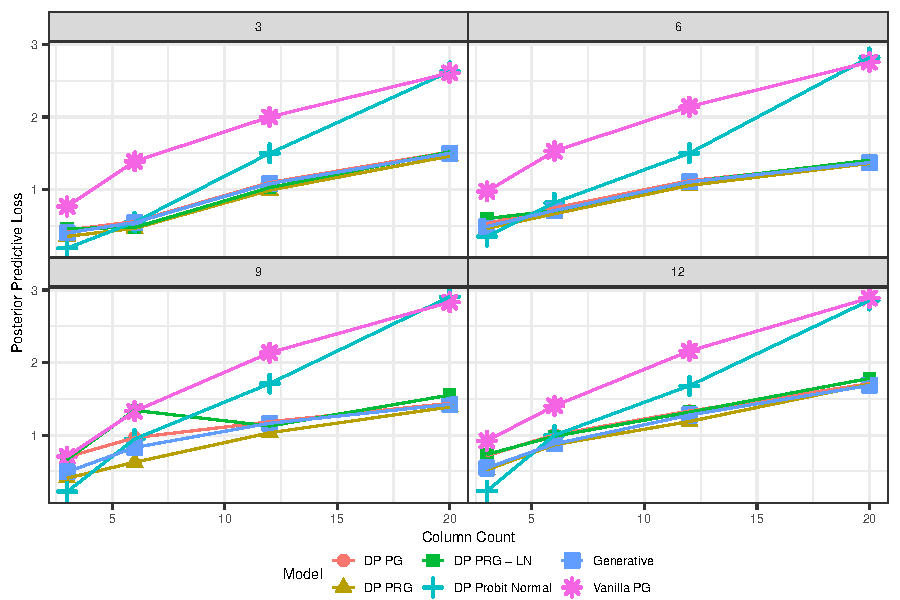
\includegraphics[width=0.45\textwidth]{./images/simulation_ppl}~
    \hfill
    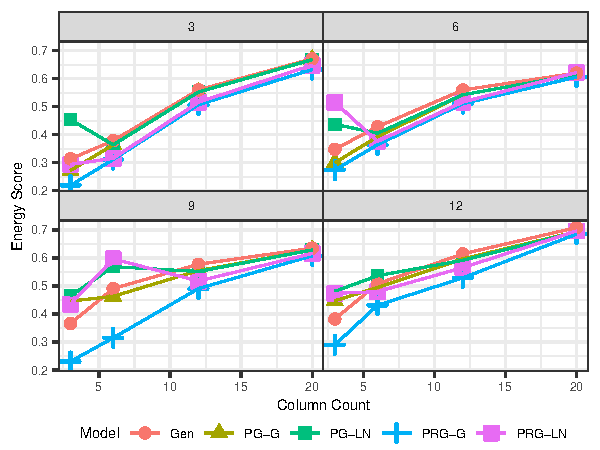
\includegraphics[width=0.45\textwidth]{./images/simulation_es}~
  \end{center}
\end{frame}

\subsection{Integrated Vapor Transport}
\begin{frame}
  \frametitle{Integrated Vapor Transport}
  \begin{center}
    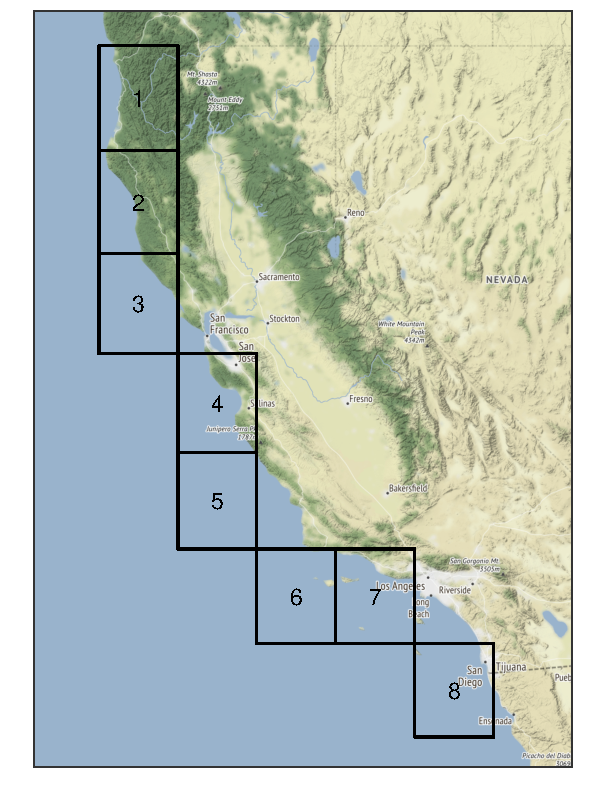
\includegraphics[width=0.33\textwidth]{./images/erai_grid}~
    \;\;\;\;\;\;
    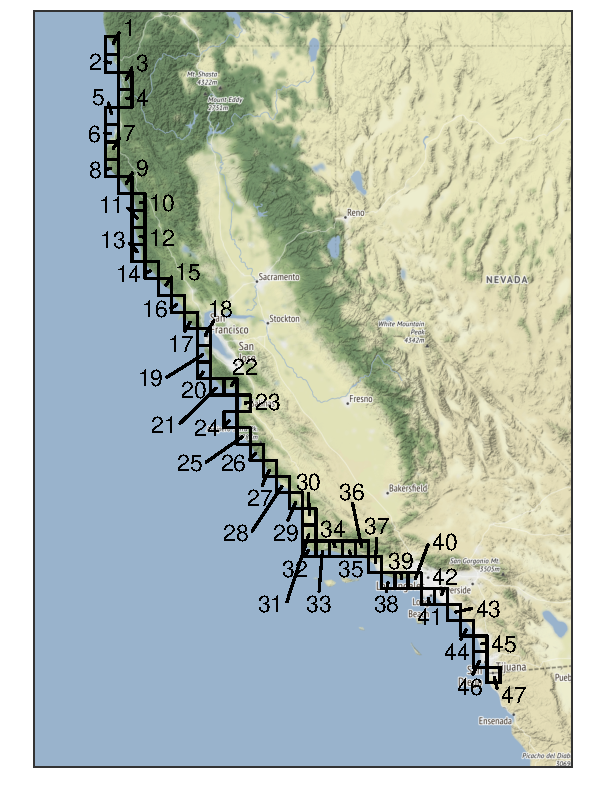
\includegraphics[width=0.33\textwidth]{./images/era5_grid}~
  \end{center}
\end{frame}

\begin{frame}
  \frametitle{Integrated Vapor Transport}
  \begin{center}
    
\begin{tabular}{ccccc}
\toprule
\multicolumn{1}{c}{ } & \multicolumn{2}{c}{dim = 8} & \multicolumn{2}{c}{dim = 47} \\
\cmidrule(l{3pt}r{3pt}){2-3} \cmidrule(l{3pt}r{3pt}){4-5}
Model & PPL & ES & PPL & ES\\
\midrule
PRG & 0.195 & 0.170 & 1.623 & 0.675\\
PRG-LN & 0.232 & 0.192 & 1.400 & 0.582\\
PG & 0.787 & 0.418 & 5.040 & 1.374\\
\bottomrule
\end{tabular}
  \end{center}
\end{frame}

\section{Conclusion}

\begin{frame}
  \begin{center}
    
\includegraphics[width=0.6\textwidth]{./images/fin}
  \end{center}
\end{frame}



\end{document}
